\begin{flushright}
    در قسمت قبل دیدیم که برای ذخیره‌سازی اطلاعات می‌توان از روش‌های مختلفی استفاده کنیم.
    با توجه به این موضوع می‌توانیم انتزاعی دیگر به نام فایل سیستم معرفی کنیم.

فایل سیستم‌ها انواع مختلفی دارند شکل زیر نمونه‌هایی از این نوع فایل‌سیستم‌ها است.

    \begin{figure}[H]
        \centering
        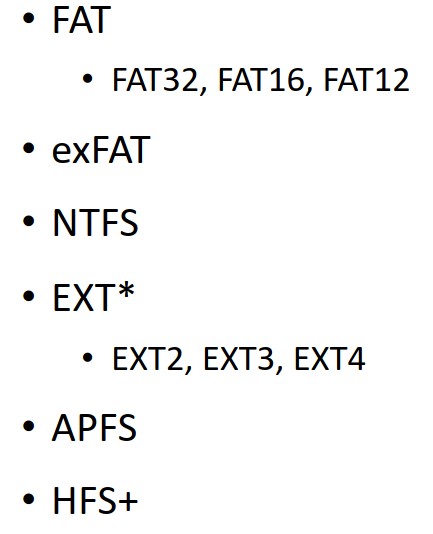
\includegraphics[width=0.2\textwidth]{source/file-system-examples}
        \caption{انواع فایل سیستم‌ها}
        \label{fig:file-system-examples}
    \end{figure}

    در ادامه بحث به فایل سیستم FAT اشاره خواهیم کرد.

\subsubject{FAT}{files/sub-file-system/FAT}
\end{flushright}